\documentclass[11pt]{article}
\usepackage[margin=1in]{geometry}
\usepackage{amsmath,amssymb}
\usepackage{booktabs}
\usepackage{graphicx}
\usepackage{float}
\usepackage[hidelinks]{hyperref}
\graphicspath{{pop_sweep/figures/}}
\title{Hard AbsTopK input gate on MNIST: hard backward against DUST steps at five population sizes}
\author{}
\date{2026-10-22}

\begin{document}
\maketitle

\section{Setup}

Two-layer MLP on MNIST, $z = W_2\,\mathrm{ReLU}(W_1 x' + b_1) + b_2$ with
hidden width 1024, where $x' = \operatorname{AbsTopK}_K(e^{g} \odot x)$ keeps
the $K$ entries of largest magnitude of the rescaled input; $g \in
\mathbb{R}^{784}$ is trainable from $0$, pixels are in $[0, 1]$.  AdamW,
learning rate $10^{-3}$ with 100 warmup steps and a cosine decay to $10^{-4}$
over 5000 steps of batch 128, no weight decay, no gradient clipping, seed 1337
(the same data order and initialization for every run of a given $K$).

\textbf{Hard}: the backward passes the hard mask, so $g_n$ moves only through
samples whose support contains pixel $n$.  \textbf{DUST}: the same gate, with
every second optimizer step a DUST step (schedule $[1, 1]$): the gate input
$u = e^{g} \odot x$ of every sample is perturbed on all 784 pixels with
$\mathcal N(0, \sigma^2)$ noise, $\sigma = 0.1$, in $P$ draws (the
population), the tail is rerun, and
$$
\hat g_t = \frac{1}{P\,\sigma\,B} \sum_{i=1}^{P} \bigl(\ell^{(i)}_t - \bar\ell_t\bigr)\, a^{(i)}_t,
\qquad
\hat G_g = \sum_t \hat g_t \odot e^{g} \odot x_t
$$
is applied to $g$ by the shared optimizer; nothing else moves on a DUST step,
so a DUST run has 2500 hard steps for $W_1, W_2$ against 5000 for the hard
run.  $K \in \{4, 8, 16, 32\}$, $P \in \{128, 512, 2000, 8000, 32000\}$.
Training CE is the clean hard forward on both kinds of step; test CE and
accuracy are the deterministic hard forward on the 10\,000 test images.

\section{Results}

RESULTS-PLACEHOLDER

\begin{figure}[H]
\centering
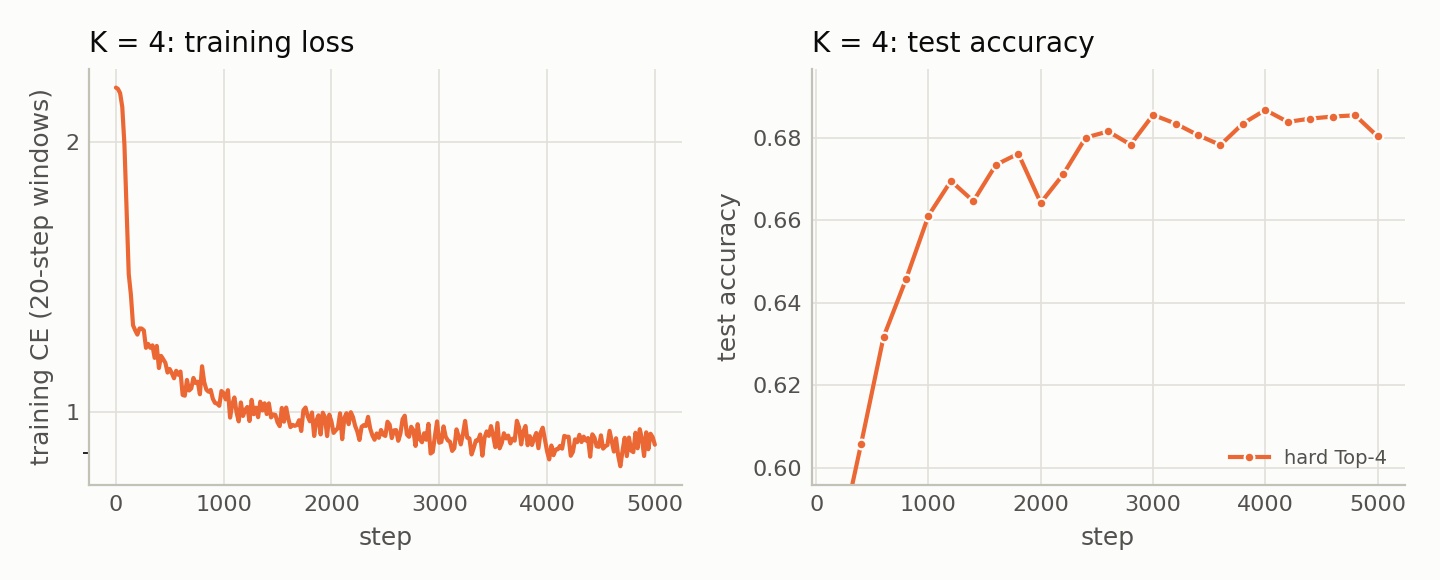
\includegraphics[width=\linewidth]{curves_k4.png}
\caption{$K = 4$: training CE (left, log scale, 20-step window means) and test accuracy (right, every 200 steps) for the hard backward and DUST at five populations.}
\label{fig:k4}
\end{figure}

\begin{figure}[H]
\centering
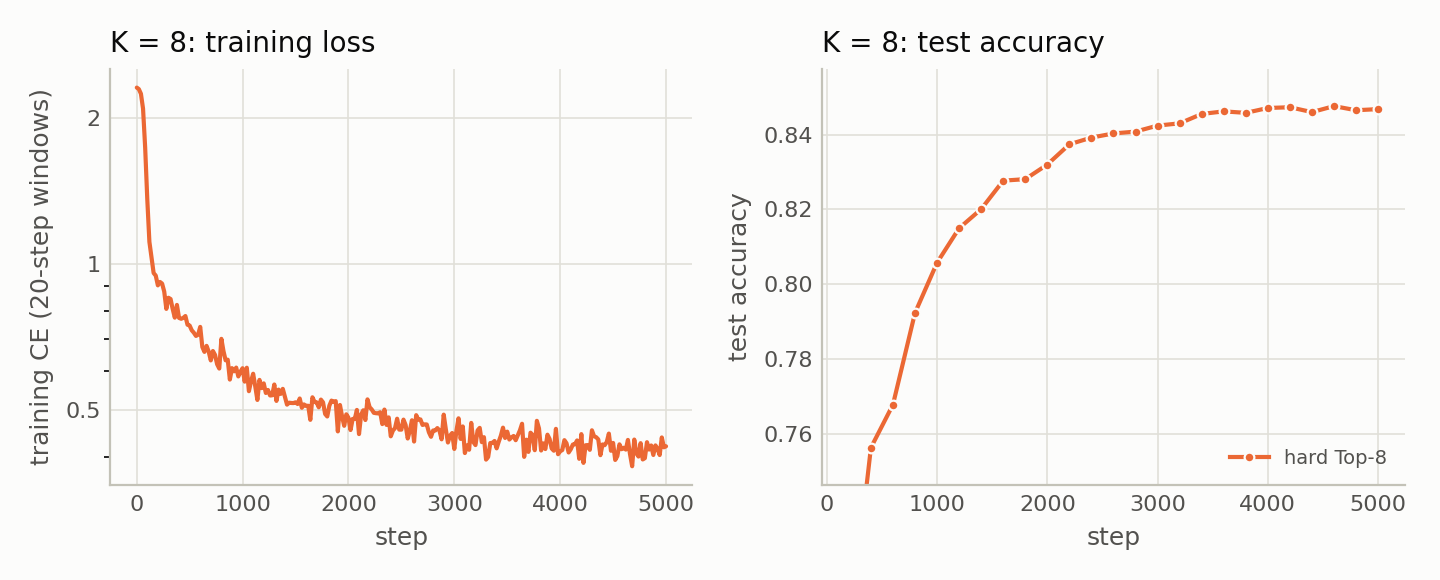
\includegraphics[width=\linewidth]{curves_k8.png}
\caption{$K = 8$: training CE (left, log scale, 20-step window means) and test accuracy (right, every 200 steps) for the hard backward and DUST at five populations.}
\label{fig:k8}
\end{figure}

\begin{figure}[H]
\centering
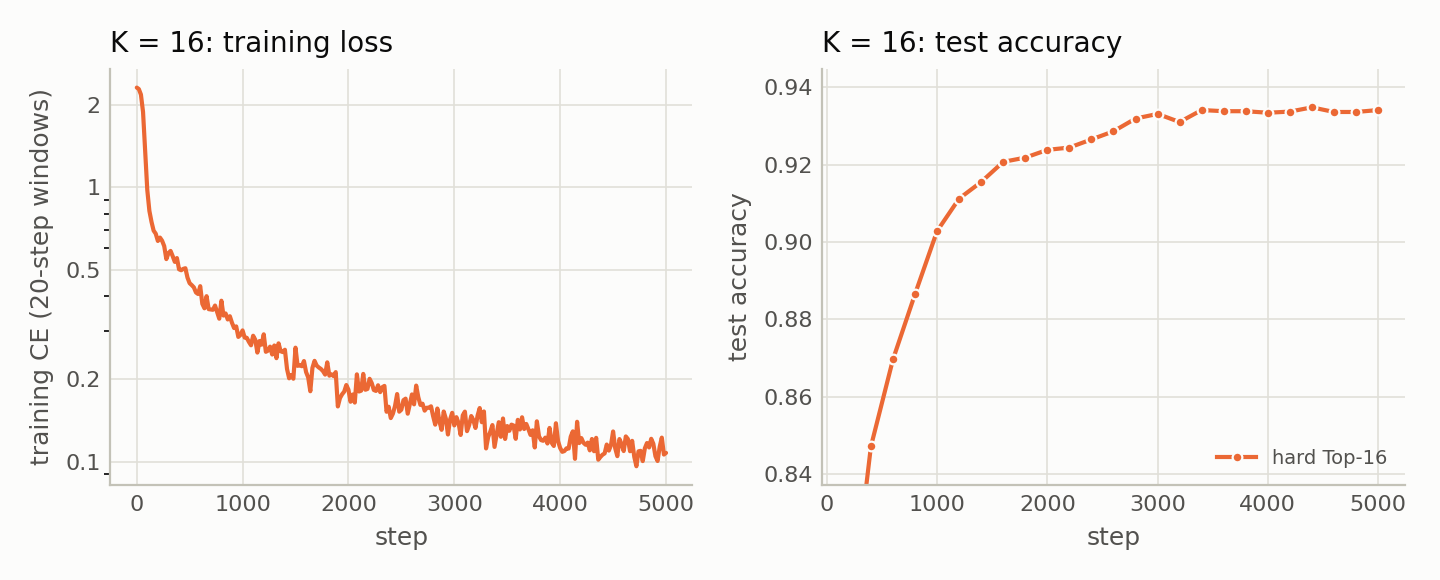
\includegraphics[width=\linewidth]{curves_k16.png}
\caption{$K = 16$: training CE (left, log scale, 20-step window means) and test accuracy (right, every 200 steps) for the hard backward and DUST at five populations.}
\label{fig:k16}
\end{figure}

\begin{figure}[H]
\centering
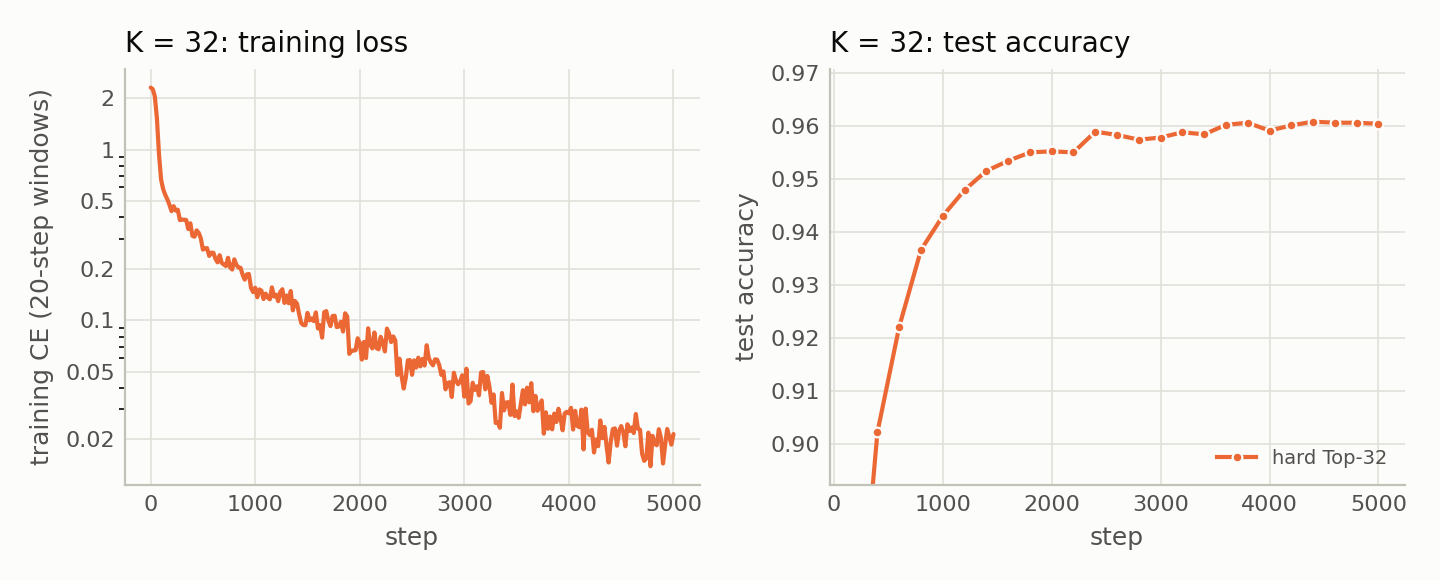
\includegraphics[width=\linewidth]{curves_k32.png}
\caption{$K = 32$: training CE (left, log scale, 20-step window means) and test accuracy (right, every 200 steps) for the hard backward and DUST at five populations.}
\label{fig:k32}
\end{figure}

\begin{table}[H]
\centering
\caption{$K = 4$: values at the final step (5000). Training CE is the mean of the last 20-step window of the clean hard forward; test CE and accuracy are the deterministic hard forward on the 10\,000 test images.}
\label{tab:k4}
\begin{tabular}{llrrr}
\toprule
    method & population & train CE & test CE & test acc (\%) \\
\midrule
    hard Top-$K$ & -- & 0.9186 & 0.9305 & 68.03 \\
\bottomrule
\end{tabular}
\end{table}

\begin{table}[H]
\centering
\caption{$K = 8$: values at the final step (5000). Training CE is the mean of the last 20-step window of the clean hard forward; test CE and accuracy are the deterministic hard forward on the 10\,000 test images.}
\label{tab:k8}
\begin{tabular}{llrrr}
\toprule
    method & population & train CE & test CE & test acc (\%) \\
\midrule
    hard Top-$K$ & -- & 0.4203 & 0.4834 & 84.68 \\
\bottomrule
\end{tabular}
\end{table}

\begin{table}[H]
\centering
\caption{$K = 16$: values at the final step (5000). Training CE is the mean of the last 20-step window of the clean hard forward; test CE and accuracy are the deterministic hard forward on the 10\,000 test images.}
\label{tab:k16}
\begin{tabular}{llrrr}
\toprule
    method & population & train CE & test CE & test acc (\%) \\
\midrule
    hard Top-$K$ & -- & 0.1077 & 0.2174 & 93.41 \\
\bottomrule
\end{tabular}
\end{table}

\begin{table}[H]
\centering
\caption{$K = 32$: values at the final step (5000). Training CE is the mean of the last 20-step window of the clean hard forward; test CE and accuracy are the deterministic hard forward on the 10\,000 test images.}
\label{tab:k32}
\begin{tabular}{llrrr}
\toprule
    method & population & train CE & test CE & test acc (\%) \\
\midrule
    hard Top-$K$ & -- & 0.0215 & 0.1466 & 96.05 \\
\bottomrule
\end{tabular}
\end{table}


\end{document}
